% chktex-file 13

\documentclass{article}
\usepackage{amsmath}
\usepackage{hyperref}
\usepackage{xcolor}
\usepackage{ulem}
\usepackage{graphicx}
\usepackage[margin=0.75in]{geometry}

\graphicspath{ {./images/} }

\definecolor{darkblue}{rgb}{0, 0, 20}

\hypersetup{
    colorlinks=true,
    urlcolor=darkblue,
    linkcolor=blue,
    filecolor=magenta,
    citecolor=blue,
}

\title{HandDiff: 3D Hand Pose Estimation with Diffusion on Image-Point Cloud}
\author{Wencan Cheng, Hao Tang, Luc Van Gool, Jong Hwan Ko}
\date{}
\setlength{\parindent}{0pt}

\begin{document}

\maketitle

\begin{center}\textbf{Accepted for CVPR 2024 (\href{https://arxiv.org/pdf/2404.03159}{Paper}) (\href{https://github.com/cwc1260/HandDiff}{GitHub})}\end{center}

This paper introduces a new 3d hand pose estimation model based on diffusion models. The model uses depth images and hand-shaped 3D point clouds, samples a random set of joint positions from a normal distribution and then, iteratively denoises the hand poses and estimates joint locations.

\section*{Motivation}

Self-occlusions is a common problem for hand pose as finger joints are often occluded. Also, previous 3D diffusion models is that they rely on global features and overlook local details. Another issue of 3D diffusion models is that they are permutation-equivariant which limits their ability to distinguish between joints.

\begin{center}
    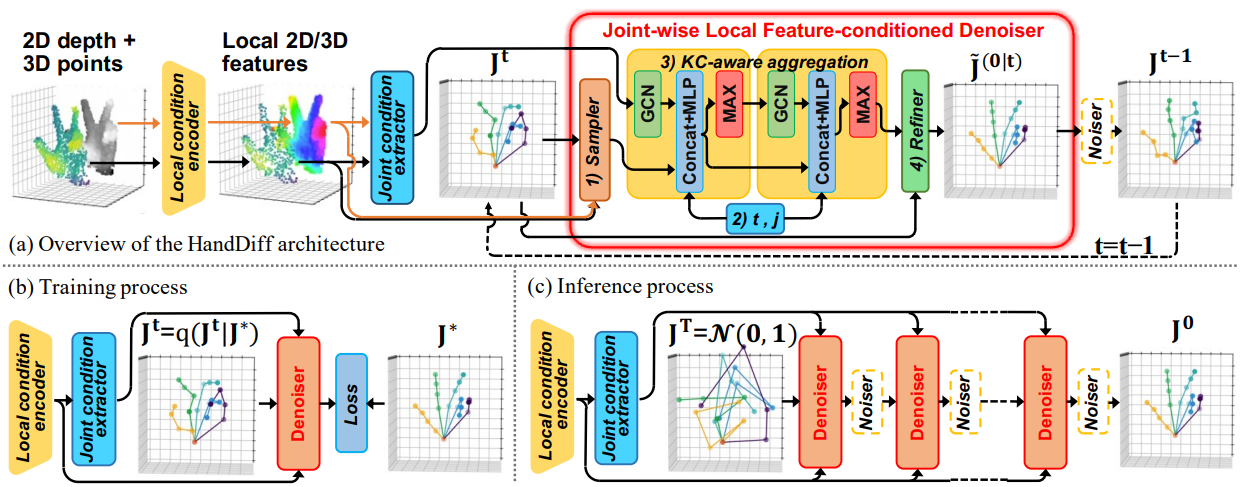
\includegraphics[scale=0.4]{handdiff-1.png}
\end{center}

\section*{Method}

\begin{enumerate}
    \item \textbf{Joint-wise Condition Extraction}
    
    The ConvNeXt-based encoder processes the depth image to generate a 2D local visual feature map and a 2D global vector. The PointNet++ encoder processes the 3D point cloud to gemerate 3D local geometric features and a 3D global vector. The global vectors are concatenated to form a single global representation. The global representation is passed through three layers of Bias-Induced Layers (BIL) to generate joint-wise embeddings (joint-wise conditions).

    \item \textbf{Joint-wise Local Feature-conditioned Denoiser}
    
    The denoiser starts with a set of joint coordinates that are randomly sampled from a Gaussian distribution. At each time step, the denoiser samples local features around each noisy joint in both 2D and 3D spaces, encodes the joint index and timestep into embeddings, aggregates local features with joint-wise conditions using a kinematic-aware GCN block, and outputs the refined joint coordinates for the next step.
\end{enumerate}

\begin{center}
    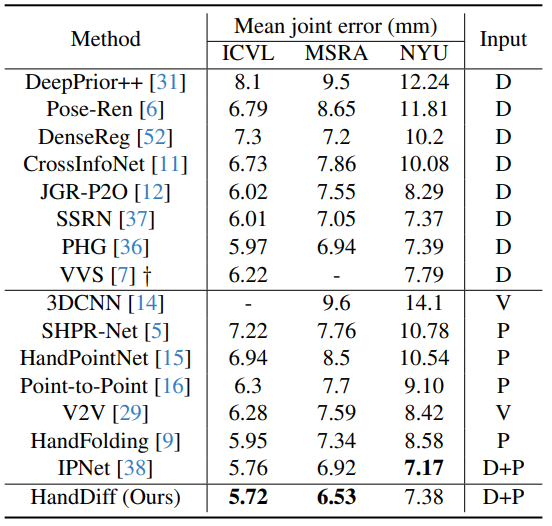
\includegraphics[scale=0.4]{handdiff-2.png}
\end{center}

\section*{Limitations}

\begin{enumerate}
    \item The model's performance plateaus after 5 timesteps which limits further optimization.
    \item The model is unable to handle scenarios with interacting hands and focuses on single-hand samples, as stated in the conclusion.
\end{enumerate}

\end{document}